\section{Problema 2}


Los estimadores de máxima verosimilitud tienen propiedades interesantes cuando se trabaja con muestras grandes. Suponga que $t(\theta)$ es una función derivable en $\theta$. Por la propiedad de invarianza, se tiene que si $\hat{\theta}$ es el MLE de $\theta$, entonces el MLE de $t(\theta)$ está dada por $t(\hat{\theta}) .$ En algunas condiciones de regularidad que se cumplen para las distribuciones que se consideren, $t(\hat{\theta})$ es un estimador consistente para $t(\theta) .$ Además, para tamaño de muestras grandes,
$$
Z=\frac{t(\hat{\theta})-t(\theta)}{\sqrt{\left[\frac{\partial t(\theta)}{\partial \theta}\right]^{2} \Big/ n E\left[-\frac{\partial^{2} \ln [f(Y \mid \theta)]}{\partial \theta^{2}}\right]}}
$$
tiene aproximandamente una distribución normal estándar, donde $f(Y \mid \theta)$ es la función densidad correspondiente a la distribución continua de interés, evaluada en el valor aleatorio Y. En el caso discreto, el resultado análogo se cumple con la función de probabilidad evaluada en el valor aleatorio $\mathrm{Y}$, $p(Y \mid \theta)$, se sustituye por la densidad $f(Y \mid \theta)$. 
\begin{tcolorbox}[colback=blue!15,colframe=blue!1!blue,title=Nota 1]
	Under the following conditions
\begin{center}
	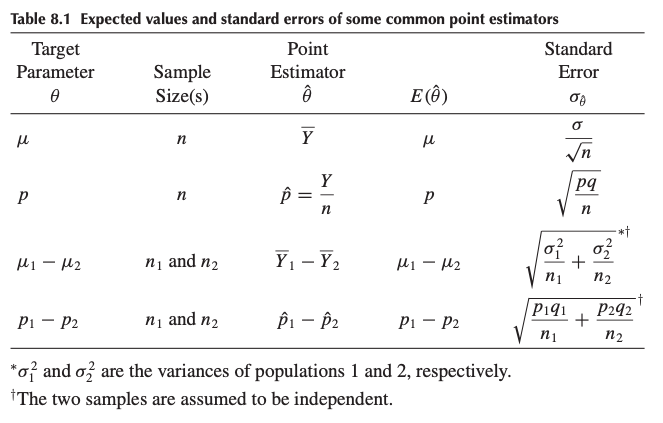
\includegraphics[scale=0.5]{/Users/rudiks/Git/Estadistica_Matematica/Parcial4/Images/Screen Shot 2021-05-23 at 16.03.22.png}
\end{center}
If the target parameter $\theta$  is $\mu, p, \mu_1 -\mu_2$, or $p_1 - p_2$, then for large samples,
$$Z=\frac{\hat{\theta}-\theta}{\sigma_{\hat{\theta}} }$$
possesses approximately a standard normal distribution. Consequently, $Z=\frac{\hat{\theta}-\theta}{\sigma_{\hat{\theta}} }$ forms (at least approximately) a pivotal quantity, and the pivotal method can be employed to develop confidence intervals for the target parameter $\theta$.\newline 

For interval confidence the key formula is: 
$$\hat{\theta}\pm z_{\alpha/2}\sigma_{\hat{\theta}}.$$
When $\theta=\mu$ is the target parameter, then $\hat{\theta}=\overline{Y}$ and $\sigma^2_{\hat{\theta}}=\sigma^2/n$. 
	\end{tcolorbox}

\begin{tcolorbox}[colback=blue!15,colframe=blue!1!blue,title=Nota 2]
	Por las condiciones de la nota 1, entonces, el intervalo buscado para $Z$ es: 
	$$t(\hat{\theta})\pm z_{\alpha/2}\sqrt{\left[\frac{\partial t(\theta)}{\partial \theta}\right]^{2} \Big/ n E\left[-\frac{\partial^{2} \ln [f(Y \mid \theta)]}{\partial \theta^{2}}\right]}\approx$$
	
	$$\approx t(\hat{\theta})\pm z_{\alpha/2}\sqrt{\left[\frac{\partial t(\hat{\theta})}{\partial \hat{\theta}}\right]^{2} \Big/ n E\left[-\frac{\partial^{2} \ln [f(Y \mid \hat{\theta})]}{\partial \hat{\theta}^{2}}\right]}$$
\end{tcolorbox}


En el caso particular, para una variable aleatoria con distribución de Bernoulli, $p(y \mid p)=$ $p^{y}(1-p)^{1-y}$, donde $\mathrm{y}=0,1 .$ Si $Y_{1}, \ldots, Y_{n}$ es una muestra aleatoria de tamaño $\mathrm{n}$ de dicha distribución.

\begin{enumerate}
	\item a) Encuentre el MLE para el parámetro p.
	\begin{solution}
		Comenzamos definiendo el MLE, como: 
		\begin{tcolorbox}[colback=gray!15,colframe=black!1!black,title=Method of Maximum Likehood]
			Suppose that the likelihood function depends on k parameters $\theta_1,\theta_2,...,\theta_k$. Choose as estimates those values of the parameters that maximize the likelihood $L(y_1, y_2,..., y_n |\theta_1,\theta_2,...,\theta_k)$.
			\end{tcolorbox}
$\implies$ Usando la definición de verosimilitud: 
\begin{align*}
	p(y|p) &= L(y_1,y_2,\cdots, y_n | p) = p^y(1-p)^{1-y}, \qquad \left(y=\frac{1}{n}\sum_{i=1}^{n}y_i\right)\\
	\ln\left[	p(y|p)\right] &= \ln\left[ p^y(1-p)^{1-y}\right] = \ln\left[p^y\right]+\ln\left[(1-p)^{1-y}\right]\\
	&= y\ln\left[p\right]+(1-y)\ln\left[(1-p)\right]\\
	\frac{\partial\ln\left[	p(y|p)\right]}{\partial p} &= \frac{y}{p}+\frac{(1-y)}{(1-p)}(-1) = \frac{y}{p}-\frac{(1-y)}{(1-p)} \qquad (*)\\
	 \frac{\partial^2\ln\left[	p(y|p)\right]}{\partial p^2} &= -\frac{y}{p^2}-\frac{(1-y)}{(1-p)^2}\qquad \text{$(**)$ Nos ayudará en el inciso 3. c)}
\end{align*}
Igualando $(*)$ a 0: 
$$ \frac{y}{\hat{p}}-\frac{(1-y)}{(1-\hat{p})} =0\implies \hat{p}= y.$$
	\end{solution}
	\item b) Encuentre el MLE para la expresión p(1-p).
	\begin{solution}
		Bajo los supuestos usuales, el MLE de $t(p)=p(1-p)$ es $t(\hat{p})=\hat{p}(1-\hat{p})$. En donde:
		\begin{align*}
			t(p) & = p(1-p) = p-p^2\\
			\frac{dt(p)}{dp} &= 1- 2p
				\end{align*}
Igualando a 0:
$$1-2\hat{p}=0\implies \hat{p}=\frac{1}{2}.$$
		
	\end{solution}
	\item c) Construya un intervalo de confianza de $100(1-\alpha) \%$ para $\mathrm{p}(1-\mathrm{p})$, la varianza de dicha distribución (suponga una muestra grande).
	\begin{solution}
		Ahora, tómese como referencia la \textbf{Nota 2}. Aún nos falta calcular: 
		$$E\left[-\frac{\partial^{2} \ln [f(Y \mid \hat{\theta})]}{\partial \hat{\theta}^{2}}\right]=E\left[-\frac{\partial^{2} \ln [p(y \mid \hat{p})]}{\partial \hat{p}^{2}}\right]=\underbrace{E\left[-\left(-\frac{y}{p^2}-\frac{(1-y)}{(1-p)^2}\right)\right]}_{\text{$(**)$ del inciso 1 a)}}=$$
		Sabemos que $\hat{p}=y$, entonces:
		$$=\left(\frac{p}{p^2}+\frac{(1-p)}{(1-p)^2}\right)=\frac{1}{p(1-p)}.$$
		Entonces, el intervalo de confianza para $p(1-p)$, como se estableció en la \textbf{Nota 2}, se define:
		$$t(\hat{p})\pm z_{\alpha/2}\sqrt{\left[\frac{\partial t(\hat{p})}{\partial \hat{p}}\right]^{2} \Big/ n E\left[-\frac{\partial^{2} \ln [f(Y \mid \hat{p})]}{\partial \hat{p}^{2}}\right]}=$$
		$$=\hat{p}(1-\hat{p})\pm z_{\alpha/2}\sqrt{\left[1-2p\right]^{2} \Big/ n \left(\frac{1}{p(1-p)}\right)}=$$
		$$=\hat{p}(1-\hat{p})\pm z_{\alpha/2}\sqrt{\frac{\hat{p}(1-\hat{p})(1-2\hat{p})^2}{n}}.$$
	\end{solution}
\end{enumerate}
 (Valor 25 puntos).
